\documentclass[1p]{elsarticle_modified}
%\bibliographystyle{elsarticle-num}

%\usepackage[colorlinks]{hyperref}
%\usepackage{abbrmath_seonhwa} %\Abb, \Ascr, \Acal ,\Abf, \Afrak
\usepackage{amsfonts}
\usepackage{amssymb}
\usepackage{amsmath}
\usepackage{amsthm}
\usepackage{scalefnt}
\usepackage{amsbsy}
\usepackage{kotex}
\usepackage{caption}
\usepackage{subfig}
\usepackage{color}
\usepackage{graphicx}
\usepackage{xcolor} %% white, black, red, green, blue, cyan, magenta, yellow
\usepackage{float}
\usepackage{setspace}
\usepackage{hyperref}

\usepackage{tikz}
\usetikzlibrary{arrows}

\usepackage{multirow}
\usepackage{array} % fixed length table
\usepackage{hhline}

%%%%%%%%%%%%%%%%%%%%%
\makeatletter
\renewcommand*\env@matrix[1][\arraystretch]{%
	\edef\arraystretch{#1}%
	\hskip -\arraycolsep
	\let\@ifnextchar\new@ifnextchar
	\array{*\c@MaxMatrixCols c}}
\makeatother %https://tex.stackexchange.com/questions/14071/how-can-i-increase-the-line-spacing-in-a-matrix
%%%%%%%%%%%%%%%

\usepackage[normalem]{ulem}

\newcommand{\msout}[1]{\ifmmode\text{\sout{\ensuremath{#1}}}\else\sout{#1}\fi}
%SOURCE: \msout is \stkout macro in https://tex.stackexchange.com/questions/20609/strikeout-in-math-mode

\newcommand{\cancel}[1]{
	\ifmmode
	{\color{red}\msout{#1}}
	\else
	{\color{red}\sout{#1}}
	\fi
}

\newcommand{\add}[1]{
	{\color{blue}\uwave{#1}}
}

\newcommand{\replace}[2]{
	\ifmmode
	{\color{red}\msout{#1}}{\color{blue}\uwave{#2}}
	\else
	{\color{red}\sout{#1}}{\color{blue}\uwave{#2}}
	\fi
}

\newcommand{\Sol}{\mathcal{S}} %segment
\newcommand{\D}{D} %diagram
\newcommand{\A}{\mathcal{A}} %arc


%%%%%%%%%%%%%%%%%%%%%%%%%%%%%5 test

\def\sl{\operatorname{\textup{SL}}(2,\Cbb)}
\def\psl{\operatorname{\textup{PSL}}(2,\Cbb)}
\def\quan{\mkern 1mu \triangleright \mkern 1mu}

\theoremstyle{definition}
\newtheorem{thm}{Theorem}[section]
\newtheorem{prop}[thm]{Proposition}
\newtheorem{lem}[thm]{Lemma}
\newtheorem{ques}[thm]{Question}
\newtheorem{cor}[thm]{Corollary}
\newtheorem{defn}[thm]{Definition}
\newtheorem{exam}[thm]{Example}
\newtheorem{rmk}[thm]{Remark}
\newtheorem{alg}[thm]{Algorithm}

\newcommand{\I}{\sqrt{-1}}
\begin{document}

%\begin{frontmatter}
%
%\title{Boundary parabolic representations of knots up to 8 crossings}
%
%%% Group authors per affiliation:
%\author{Yunhi Cho} 
%\address{Department of Mathematics, University of Seoul, Seoul, Korea}
%\ead{yhcho@uos.ac.kr}
%
%
%\author{Seonhwa Kim} %\fnref{s_kim}}
%\address{Center for Geometry and Physics, Institute for Basic Science, Pohang, 37673, Korea}
%\ead{ryeona17@ibs.re.kr}
%
%\author{Hyuk Kim}
%\address{Department of Mathematical Sciences, Seoul National University, Seoul 08826, Korea}
%\ead{hyukkim@snu.ac.kr}
%
%\author{Seokbeom Yoon}
%\address{Department of Mathematical Sciences, Seoul National University, Seoul, 08826,  Korea}
%\ead{sbyoon15@snu.ac.kr}
%
%\begin{abstract}
%We find all boundary parabolic representation of knots up to 8 crossings.
%
%\end{abstract}
%\begin{keyword}
%    \MSC[2010] 57M25 
%\end{keyword}
%
%\end{frontmatter}

%\linenumbers
%\tableofcontents
%
\newcommand\colored[1]{\textcolor{white}{\rule[-0.35ex]{0.8em}{1.4ex}}\kern-0.8em\color{red} #1}%
%\newcommand\colored[1]{\textcolor{white}{ #1}\kern-2.17ex	\textcolor{white}{ #1}\kern-1.81ex	\textcolor{white}{ #1}\kern-2.15ex\color{red}#1	}

{\Large $\underline{12a_{0689}~(K12a_{0689})}$}

\setlength{\tabcolsep}{10pt}
\renewcommand{\arraystretch}{1.6}
\vspace{1cm}\begin{tabular}{m{100pt}>{\centering\arraybackslash}m{274pt}}
\multirow{5}{120pt}{
	\centering
	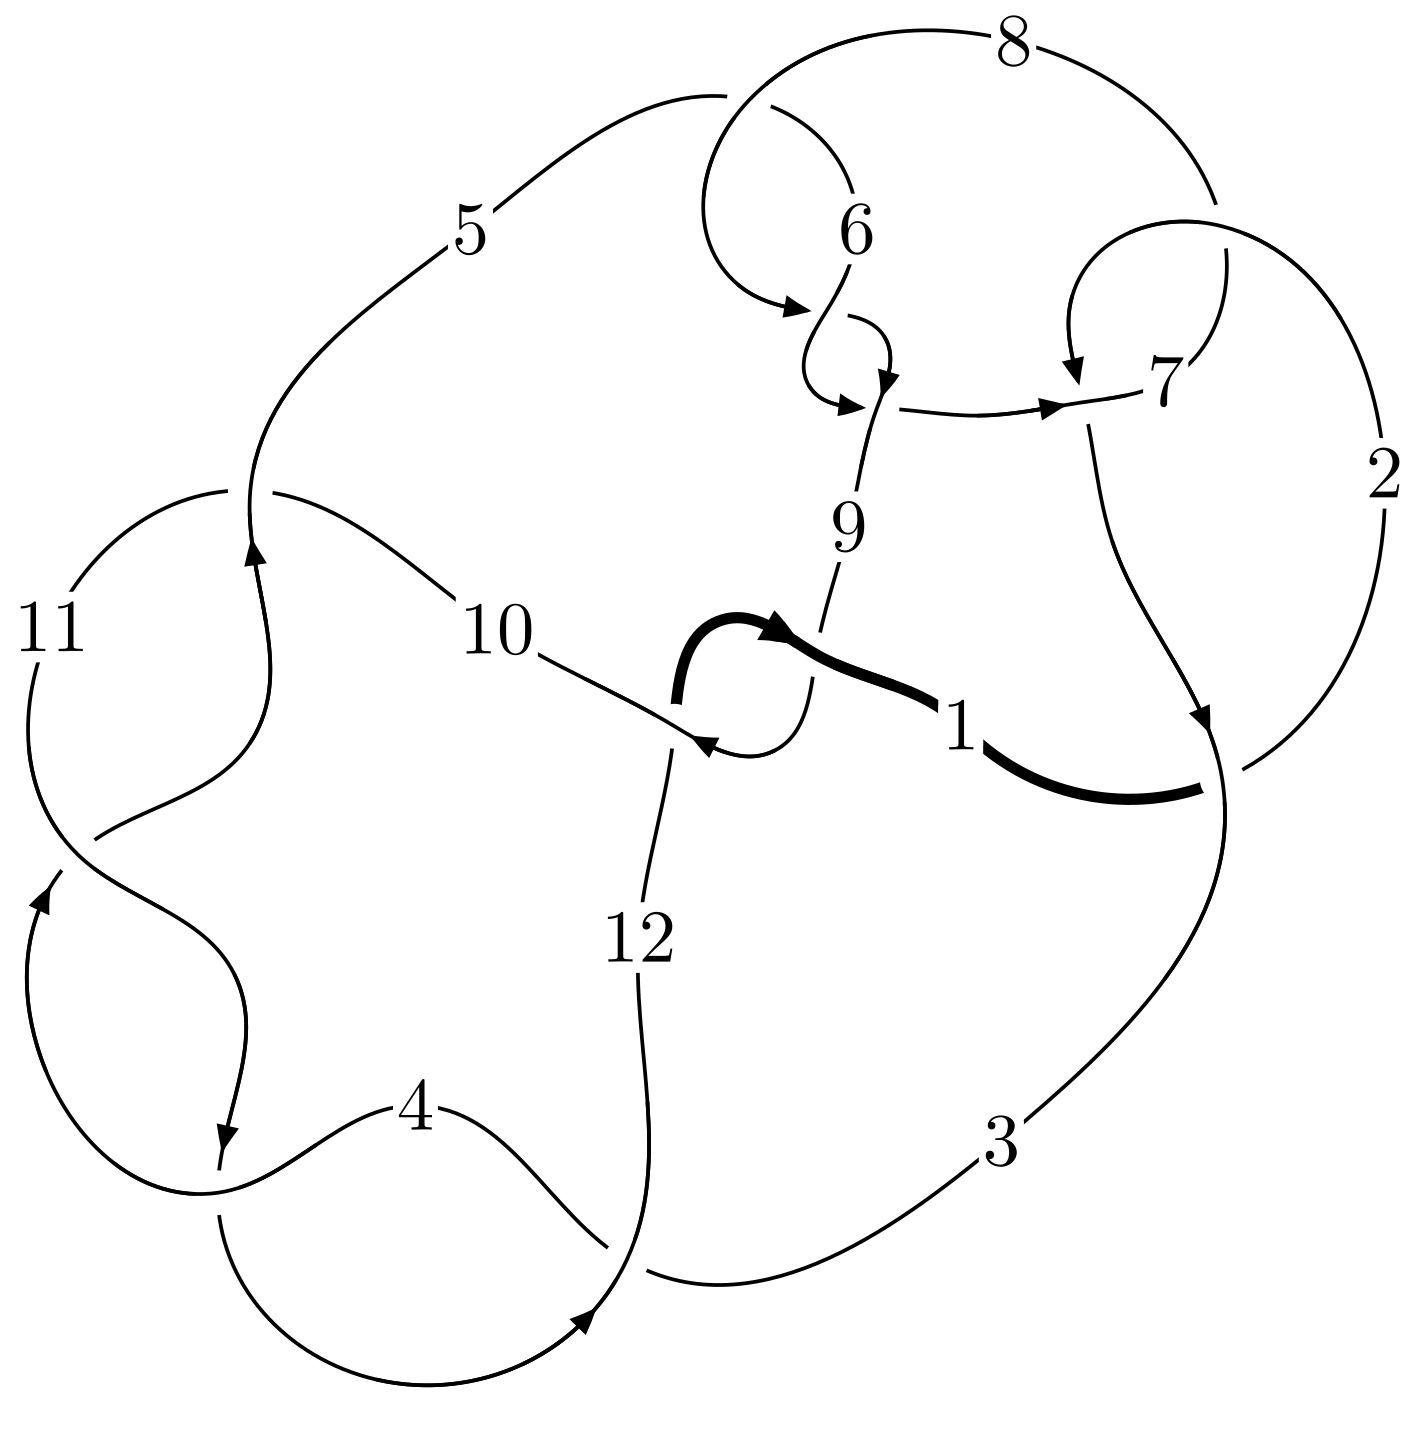
\includegraphics[width=112pt]{../../../GIT/diagram.site/Diagrams/png/1490_12a_0689.png}\\
\ \ \ A knot diagram\footnotemark}&
\allowdisplaybreaks
\textbf{Linearized knot diagam} \\
\cline{2-2}
 &
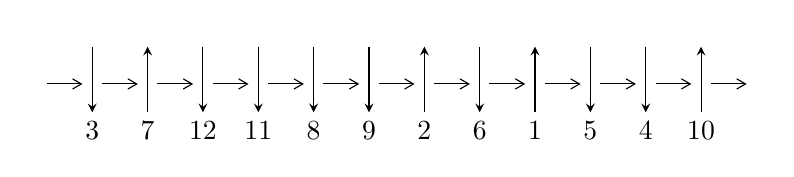
\begin{tikzpicture}[x=20pt, y=17pt]
	% nodes
	\node (C0) at (0, 0) {};
	\node (C1) at (1, 0) {};
	\node (C1U) at (1, +1) {};
	\node (C1D) at (1, -1) {3};

	\node (C2) at (2, 0) {};
	\node (C2U) at (2, +1) {};
	\node (C2D) at (2, -1) {7};

	\node (C3) at (3, 0) {};
	\node (C3U) at (3, +1) {};
	\node (C3D) at (3, -1) {12};

	\node (C4) at (4, 0) {};
	\node (C4U) at (4, +1) {};
	\node (C4D) at (4, -1) {11};

	\node (C5) at (5, 0) {};
	\node (C5U) at (5, +1) {};
	\node (C5D) at (5, -1) {8};

	\node (C6) at (6, 0) {};
	\node (C6U) at (6, +1) {};
	\node (C6D) at (6, -1) {9};

	\node (C7) at (7, 0) {};
	\node (C7U) at (7, +1) {};
	\node (C7D) at (7, -1) {2};

	\node (C8) at (8, 0) {};
	\node (C8U) at (8, +1) {};
	\node (C8D) at (8, -1) {6};

	\node (C9) at (9, 0) {};
	\node (C9U) at (9, +1) {};
	\node (C9D) at (9, -1) {1};

	\node (C10) at (10, 0) {};
	\node (C10U) at (10, +1) {};
	\node (C10D) at (10, -1) {5};

	\node (C11) at (11, 0) {};
	\node (C11U) at (11, +1) {};
	\node (C11D) at (11, -1) {4};

	\node (C12) at (12, 0) {};
	\node (C12U) at (12, +1) {};
	\node (C12D) at (12, -1) {10};
	\node (C13) at (13, 0) {};

	% arrows
	\draw[->,>={angle 60}]
	(C0) edge (C1) (C1) edge (C2) (C2) edge (C3) (C3) edge (C4) (C4) edge (C5) (C5) edge (C6) (C6) edge (C7) (C7) edge (C8) (C8) edge (C9) (C9) edge (C10) (C10) edge (C11) (C11) edge (C12) (C12) edge (C13) ;	\draw[->,>=stealth]
	(C1U) edge (C1D) (C2D) edge (C2U) (C3U) edge (C3D) (C4U) edge (C4D) (C5U) edge (C5D) (C6U) edge (C6D) (C7D) edge (C7U) (C8U) edge (C8D) (C9D) edge (C9U) (C10U) edge (C10D) (C11U) edge (C11D) (C12D) edge (C12U) ;
	\end{tikzpicture} \\
\hhline{~~} \\& 
\textbf{Solving Sequence} \\ \cline{2-2} 
 &
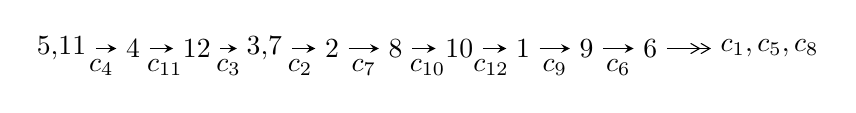
\begin{tikzpicture}[x=23pt, y=7pt]
	% node
	\node (A0) at (-1/8, 0) {5,11};
	\node (A1) at (1, 0) {4};
	\node (A2) at (2, 0) {12};
	\node (A3) at (49/16, 0) {3,7};
	\node (A4) at (33/8, 0) {2};
	\node (A5) at (41/8, 0) {8};
	\node (A6) at (49/8, 0) {10};
	\node (A7) at (57/8, 0) {1};
	\node (A8) at (65/8, 0) {9};
	\node (A9) at (73/8, 0) {6};
	\node (C1) at (1/2, -1) {$c_{4}$};
	\node (C2) at (3/2, -1) {$c_{11}$};
	\node (C3) at (5/2, -1) {$c_{3}$};
	\node (C4) at (29/8, -1) {$c_{2}$};
	\node (C5) at (37/8, -1) {$c_{7}$};
	\node (C6) at (45/8, -1) {$c_{10}$};
	\node (C7) at (53/8, -1) {$c_{12}$};
	\node (C8) at (61/8, -1) {$c_{9}$};
	\node (C9) at (69/8, -1) {$c_{6}$};
	\node (A10) at (11, 0) {$c_{1},c_{5},c_{8}$};

	% edge
	\draw[->,>=stealth]	
	(A0) edge (A1) (A1) edge (A2) (A2) edge (A3) (A3) edge (A4) (A4) edge (A5) (A5) edge (A6) (A6) edge (A7) (A7) edge (A8) (A8) edge (A9) ;
	\draw[->>,>={angle 60}]	
	(A9) edge (A10);
\end{tikzpicture} \\ 

\end{tabular} \\

\footnotetext{
The image of knot diagram is generated by the software ``\textbf{Draw programme}" developed by Andrew Bartholomew(\url{http://www.layer8.co.uk/maths/draw/index.htm\#Running-draw}), where we modified some parts for our purpose(\url{https://github.com/CATsTAILs/LinksPainter}).
}\phantom \\ \newline 
\centering \textbf{Ideals for irreducible components\footnotemark of $X_{\text{par}}$} 
 
\begin{align*}
I^u_{1}&=\langle 
u^{61}- u^{60}+\cdots+b-1,\;u^{64}-2 u^{63}+\cdots+a+2,\;u^{65}-2 u^{64}+\cdots+u-1\rangle \\
I^u_{2}&=\langle 
b-1,\;u^3+u^2+a+3 u+1,\;u^4+u^3+3 u^2+2 u+1\rangle \\
\\
\end{align*}
\raggedright * 2 irreducible components of $\dim_{\mathbb{C}}=0$, with total 69 representations.\\
\footnotetext{All coefficients of polynomials are rational numbers. But the coefficients are sometimes approximated in decimal forms when there is not enough margin.}
\newpage
\renewcommand{\arraystretch}{1}
\centering \section*{I. $I^u_{1}= \langle u^{61}- u^{60}+\cdots+b-1,\;u^{64}-2 u^{63}+\cdots+a+2,\;u^{65}-2 u^{64}+\cdots+u-1 \rangle$}
\flushleft \textbf{(i) Arc colorings}\\
\begin{tabular}{m{7pt} m{180pt} m{7pt} m{180pt} }
\flushright $a_{5}=$&$\begin{pmatrix}1\\0\end{pmatrix}$ \\
\flushright $a_{11}=$&$\begin{pmatrix}0\\u\end{pmatrix}$ \\
\flushright $a_{4}=$&$\begin{pmatrix}1\\- u^2\end{pmatrix}$ \\
\flushright $a_{12}=$&$\begin{pmatrix}- u\\u^3+u\end{pmatrix}$ \\
\flushright $a_{3}=$&$\begin{pmatrix}u^2+1\\- u^4-2 u^2\end{pmatrix}$ \\
\flushright $a_{7}=$&$\begin{pmatrix}- u^{64}+2 u^{63}+\cdots-4 u-2\\- u^{61}+u^{60}+\cdots+2 u+1\end{pmatrix}$ \\
\flushright $a_{2}=$&$\begin{pmatrix}- u^{11}-6 u^9-12 u^7-8 u^5- u^3-2 u\\u^{13}+7 u^{11}+17 u^9+16 u^7+6 u^5+5 u^3+u\end{pmatrix}$ \\
\flushright $a_{8}=$&$\begin{pmatrix}- u^{64}+2 u^{63}+\cdots-3 u-1\\- u^{61}+u^{60}+\cdots+u+1\end{pmatrix}$ \\
\flushright $a_{10}=$&$\begin{pmatrix}u\\u\end{pmatrix}$ \\
\flushright $a_{1}=$&$\begin{pmatrix}u^5+2 u^3- u\\u^5+3 u^3+u\end{pmatrix}$ \\
\flushright $a_{9}=$&$\begin{pmatrix}u^9+4 u^7+3 u^5-2 u^3+u\\u^9+5 u^7+7 u^5+2 u^3+u\end{pmatrix}$ \\
\flushright $a_{6}=$&$\begin{pmatrix}- u^{64}+2 u^{63}+\cdots-3 u-1\\- u^{61}+u^{60}+\cdots+2 u+1\end{pmatrix}$\\&\end{tabular}
\flushleft \textbf{(ii) Obstruction class $= -1$}\\~\\
\flushleft \textbf{(iii) Cusp Shapes $= - u^{64}+2 u^{63}+\cdots-10 u-3$}\\~\\
\newpage\renewcommand{\arraystretch}{1}
\flushleft \textbf{(iv) u-Polynomials at the component}\newline \\
\begin{tabular}{m{50pt}|m{274pt}}
Crossings & \hspace{64pt}u-Polynomials at each crossing \\
\hline $$\begin{aligned}c_{1}\end{aligned}$$&$\begin{aligned}
&u^{65}+27 u^{64}+\cdots-1984 u-256
\end{aligned}$\\
\hline $$\begin{aligned}c_{2},c_{7}\end{aligned}$$&$\begin{aligned}
&u^{65}+u^{64}+\cdots+24 u+16
\end{aligned}$\\
\hline $$\begin{aligned}c_{3},c_{4},c_{10}\\c_{11}\end{aligned}$$&$\begin{aligned}
&u^{65}-2 u^{64}+\cdots+u-1
\end{aligned}$\\
\hline $$\begin{aligned}c_{5},c_{6},c_{8}\end{aligned}$$&$\begin{aligned}
&u^{65}-5 u^{64}+\cdots+u+1
\end{aligned}$\\
\hline $$\begin{aligned}c_{9},c_{12}\end{aligned}$$&$\begin{aligned}
&u^{65}+12 u^{64}+\cdots+1405 u+131
\end{aligned}$\\
\hline
\end{tabular}\\~\\
\newpage\renewcommand{\arraystretch}{1}
\flushleft \textbf{(v) Riley Polynomials at the component}\newline \\
\begin{tabular}{m{50pt}|m{274pt}}
Crossings & \hspace{64pt}Riley Polynomials at each crossing \\
\hline $$\begin{aligned}c_{1}\end{aligned}$$&$\begin{aligned}
&y^{65}+15 y^{64}+\cdots-1257472 y-65536
\end{aligned}$\\
\hline $$\begin{aligned}c_{2},c_{7}\end{aligned}$$&$\begin{aligned}
&y^{65}+27 y^{64}+\cdots-1984 y-256
\end{aligned}$\\
\hline $$\begin{aligned}c_{3},c_{4},c_{10}\\c_{11}\end{aligned}$$&$\begin{aligned}
&y^{65}+72 y^{64}+\cdots+5 y-1
\end{aligned}$\\
\hline $$\begin{aligned}c_{5},c_{6},c_{8}\end{aligned}$$&$\begin{aligned}
&y^{65}-57 y^{64}+\cdots-33 y-1
\end{aligned}$\\
\hline $$\begin{aligned}c_{9},c_{12}\end{aligned}$$&$\begin{aligned}
&y^{65}+36 y^{64}+\cdots+294081 y-17161
\end{aligned}$\\
\hline
\end{tabular}\\~\\
\newpage\flushleft \textbf{(vi) Complex Volumes and Cusp Shapes}
$$\begin{array}{c|c|c}  
\text{Solutions to }I^u_{1}& \I (\text{vol} + \sqrt{-1}CS) & \text{Cusp shape}\\
 \hline 
\begin{aligned}
u &= -0.176961 + 0.834517 I \\
a &= \phantom{-}1.40512 + 0.84371 I \\
b &= \phantom{-}0.99803 + 1.05009 I\end{aligned}
 & -1.61201 + 5.84427 I & -3.29017 - 6.41076 I \\ \hline\begin{aligned}
u &= -0.176961 - 0.834517 I \\
a &= \phantom{-}1.40512 - 0.84371 I \\
b &= \phantom{-}0.99803 - 1.05009 I\end{aligned}
 & -1.61201 - 5.84427 I & -3.29017 + 6.41076 I \\ \hline\begin{aligned}
u &= \phantom{-}0.587464 + 0.605812 I \\
a &= \phantom{-}1.99776 + 1.35416 I \\
b &= \phantom{-}1.11944 - 1.68323 I\end{aligned}
 & -6.38469 - 11.44690 I & -7.68442 + 9.11849 I \\ \hline\begin{aligned}
u &= \phantom{-}0.587464 - 0.605812 I \\
a &= \phantom{-}1.99776 - 1.35416 I \\
b &= \phantom{-}1.11944 + 1.68323 I\end{aligned}
 & -6.38469 + 11.44690 I & -7.68442 - 9.11849 I \\ \hline\begin{aligned}
u &= \phantom{-}0.562023 + 0.589176 I \\
a &= -1.70682 - 1.57560 I \\
b &= -1.43980 + 1.35021 I\end{aligned}
 & -1.08419 - 7.25640 I & -4.14361 + 8.68494 I \\ \hline\begin{aligned}
u &= \phantom{-}0.562023 - 0.589176 I \\
a &= -1.70682 + 1.57560 I \\
b &= -1.43980 - 1.35021 I\end{aligned}
 & -1.08419 + 7.25640 I & -4.14361 - 8.68494 I \\ \hline\begin{aligned}
u &= -0.434655 + 0.677483 I \\
a &= -0.76935 - 1.40090 I \\
b &= \phantom{-}0.761684 - 0.558455 I\end{aligned}
 & -3.21792 - 0.04263 I & -6.95293 - 1.05086 I \\ \hline\begin{aligned}
u &= -0.434655 - 0.677483 I \\
a &= -0.76935 + 1.40090 I \\
b &= \phantom{-}0.761684 + 0.558455 I\end{aligned}
 & -3.21792 + 0.04263 I & -6.95293 + 1.05086 I \\ \hline\begin{aligned}
u &= -0.559917 + 0.567694 I \\
a &= \phantom{-}0.51071 - 1.73794 I \\
b &= \phantom{-}0.802552 + 0.895254 I\end{aligned}
 & -4.08533 + 5.19997 I & -6.95238 - 6.01151 I \\ \hline\begin{aligned}
u &= -0.559917 - 0.567694 I \\
a &= \phantom{-}0.51071 + 1.73794 I \\
b &= \phantom{-}0.802552 - 0.895254 I\end{aligned}
 & -4.08533 - 5.19997 I & -6.95238 + 6.01151 I\\
 \hline 
 \end{array}$$\newpage$$\begin{array}{c|c|c}  
\text{Solutions to }I^u_{1}& \I (\text{vol} + \sqrt{-1}CS) & \text{Cusp shape}\\
 \hline 
\begin{aligned}
u &= \phantom{-}0.618882 + 0.492399 I \\
a &= -0.690536 - 0.334295 I \\
b &= -0.479177 - 0.103237 I\end{aligned}
 & -11.32390 - 2.09934 I & -11.90160 + 3.33110 I \\ \hline\begin{aligned}
u &= \phantom{-}0.618882 - 0.492399 I \\
a &= -0.690536 + 0.334295 I \\
b &= -0.479177 + 0.103237 I\end{aligned}
 & -11.32390 + 2.09934 I & -11.90160 - 3.33110 I \\ \hline\begin{aligned}
u &= \phantom{-}0.541988 + 0.545165 I \\
a &= \phantom{-}1.05538 + 1.71117 I \\
b &= \phantom{-}1.65899 - 0.67000 I\end{aligned}
 & -3.16680 - 2.60582 I & -8.31028 + 4.78950 I \\ \hline\begin{aligned}
u &= \phantom{-}0.541988 - 0.545165 I \\
a &= \phantom{-}1.05538 - 1.71117 I \\
b &= \phantom{-}1.65899 + 0.67000 I\end{aligned}
 & -3.16680 + 2.60582 I & -8.31028 - 4.78950 I \\ \hline\begin{aligned}
u &= -0.083204 + 0.762987 I \\
a &= -1.47229 - 0.86393 I \\
b &= -1.103520 - 0.489689 I\end{aligned}
 & \phantom{-}3.00423 + 2.37974 I & \phantom{-}3.15751 - 4.54472 I \\ \hline\begin{aligned}
u &= -0.083204 - 0.762987 I \\
a &= -1.47229 + 0.86393 I \\
b &= -1.103520 + 0.489689 I\end{aligned}
 & \phantom{-}3.00423 - 2.37974 I & \phantom{-}3.15751 + 4.54472 I \\ \hline\begin{aligned}
u &= -0.491902 + 0.580057 I \\
a &= -0.057631 + 1.353840 I \\
b &= -0.650246 - 0.287216 I\end{aligned}
 & \phantom{-}0.50199 + 2.34229 I & -0.41176 - 4.10900 I \\ \hline\begin{aligned}
u &= -0.491902 - 0.580057 I \\
a &= -0.057631 - 1.353840 I \\
b &= -0.650246 + 0.287216 I\end{aligned}
 & \phantom{-}0.50199 - 2.34229 I & -0.41176 + 4.10900 I \\ \hline\begin{aligned}
u &= \phantom{-}0.628694 + 0.357461 I \\
a &= -0.979961 - 0.460853 I \\
b &= \phantom{-}0.98668 + 1.61826 I\end{aligned}
 & -7.11475 + 7.31767 I & -9.69803 - 3.17801 I \\ \hline\begin{aligned}
u &= \phantom{-}0.628694 - 0.357461 I \\
a &= -0.979961 + 0.460853 I \\
b &= \phantom{-}0.98668 - 1.61826 I\end{aligned}
 & -7.11475 - 7.31767 I & -9.69803 + 3.17801 I\\
 \hline 
 \end{array}$$\newpage$$\begin{array}{c|c|c}  
\text{Solutions to }I^u_{1}& \I (\text{vol} + \sqrt{-1}CS) & \text{Cusp shape}\\
 \hline 
\begin{aligned}
u &= -0.573521 + 0.396534 I \\
a &= -1.36868 + 0.72006 I \\
b &= \phantom{-}0.700052 - 0.740111 I\end{aligned}
 & -4.58689 - 1.30630 I & -8.69876 - 0.72424 I \\ \hline\begin{aligned}
u &= -0.573521 - 0.396534 I \\
a &= -1.36868 - 0.72006 I \\
b &= \phantom{-}0.700052 + 0.740111 I\end{aligned}
 & -4.58689 + 1.30630 I & -8.69876 + 0.72424 I \\ \hline\begin{aligned}
u &= \phantom{-}0.547064 + 0.428484 I \\
a &= -0.648498 + 0.866630 I \\
b &= \phantom{-}1.39053 + 0.84768 I\end{aligned}
 & -3.51243 - 1.15687 I & -10.08026 + 3.04392 I \\ \hline\begin{aligned}
u &= \phantom{-}0.547064 - 0.428484 I \\
a &= -0.648498 - 0.866630 I \\
b &= \phantom{-}1.39053 - 0.84768 I\end{aligned}
 & -3.51243 + 1.15687 I & -10.08026 - 3.04392 I \\ \hline\begin{aligned}
u &= \phantom{-}0.584549 + 0.365784 I \\
a &= \phantom{-}1.077210 - 0.038246 I \\
b &= -1.19511 - 1.33848 I\end{aligned}
 & -1.73587 + 3.32691 I & -6.23751 - 2.52670 I \\ \hline\begin{aligned}
u &= \phantom{-}0.584549 - 0.365784 I \\
a &= \phantom{-}1.077210 + 0.038246 I \\
b &= -1.19511 + 1.33848 I\end{aligned}
 & -1.73587 - 3.32691 I & -6.23751 + 2.52670 I \\ \hline\begin{aligned}
u &= \phantom{-}0.061107 + 0.669375 I \\
a &= \phantom{-}1.86977 + 0.92766 I \\
b &= \phantom{-}1.256900 - 0.293507 I\end{aligned}
 & -0.052808 - 1.067730 I & \phantom{-}0.522323 + 0.688585 I \\ \hline\begin{aligned}
u &= \phantom{-}0.061107 - 0.669375 I \\
a &= \phantom{-}1.86977 - 0.92766 I \\
b &= \phantom{-}1.256900 + 0.293507 I\end{aligned}
 & -0.052808 + 1.067730 I & \phantom{-}0.522323 - 0.688585 I \\ \hline\begin{aligned}
u &= \phantom{-}0.12768 + 1.41720 I \\
a &= -0.219186 + 0.941667 I \\
b &= \phantom{-}0.74968 + 1.50855 I\end{aligned}
 & -1.52933 + 4.66645 I & \phantom{-0.000000 } 0 \\ \hline\begin{aligned}
u &= \phantom{-}0.12768 - 1.41720 I \\
a &= -0.219186 - 0.941667 I \\
b &= \phantom{-}0.74968 - 1.50855 I\end{aligned}
 & -1.52933 - 4.66645 I & \phantom{-0.000000 } 0\\
 \hline 
 \end{array}$$\newpage$$\begin{array}{c|c|c}  
\text{Solutions to }I^u_{1}& \I (\text{vol} + \sqrt{-1}CS) & \text{Cusp shape}\\
 \hline 
\begin{aligned}
u &= -0.549260 + 0.140873 I \\
a &= -0.771450 - 0.335665 I \\
b &= \phantom{-}0.703771 + 0.825353 I\end{aligned}
 & -4.80826 + 3.38006 I & -10.74337 - 4.24525 I \\ \hline\begin{aligned}
u &= -0.549260 - 0.140873 I \\
a &= -0.771450 + 0.335665 I \\
b &= \phantom{-}0.703771 - 0.825353 I\end{aligned}
 & -4.80826 - 3.38006 I & -10.74337 + 4.24525 I \\ \hline\begin{aligned}
u &= -0.397665 + 0.374585 I \\
a &= \phantom{-}0.879636 - 0.312320 I \\
b &= -0.225733 + 0.046292 I\end{aligned}
 & -0.161016 + 0.965316 I & -1.89057 - 5.10054 I \\ \hline\begin{aligned}
u &= -0.397665 - 0.374585 I \\
a &= \phantom{-}0.879636 + 0.312320 I \\
b &= -0.225733 - 0.046292 I\end{aligned}
 & -0.161016 - 0.965316 I & -1.89057 + 5.10054 I \\ \hline\begin{aligned}
u &= \phantom{-}0.10989 + 1.46208 I \\
a &= \phantom{-}0.189540 - 1.294750 I \\
b &= -0.77445 - 1.43903 I\end{aligned}
 & \phantom{-}4.08220 + 1.01313 I & \phantom{-0.000000 } 0 \\ \hline\begin{aligned}
u &= \phantom{-}0.10989 - 1.46208 I \\
a &= \phantom{-}0.189540 + 1.294750 I \\
b &= -0.77445 + 1.43903 I\end{aligned}
 & \phantom{-}4.08220 - 1.01313 I & \phantom{-0.000000 } 0 \\ \hline\begin{aligned}
u &= -0.12743 + 1.47880 I \\
a &= -0.875843 + 0.046170 I \\
b &= \phantom{-}0.504534 - 0.571892 I\end{aligned}
 & \phantom{-}1.48337 + 1.06097 I & \phantom{-0.000000 } 0 \\ \hline\begin{aligned}
u &= -0.12743 - 1.47880 I \\
a &= -0.875843 - 0.046170 I \\
b &= \phantom{-}0.504534 + 0.571892 I\end{aligned}
 & \phantom{-}1.48337 - 1.06097 I & \phantom{-0.000000 } 0 \\ \hline\begin{aligned}
u &= \phantom{-}0.13453 + 1.49947 I \\
a &= \phantom{-}0.60759 + 1.59619 I \\
b &= \phantom{-}1.18048 + 1.16499 I\end{aligned}
 & \phantom{-}2.82349 - 3.48654 I & \phantom{-0.000000 } 0 \\ \hline\begin{aligned}
u &= \phantom{-}0.13453 - 1.49947 I \\
a &= \phantom{-}0.60759 - 1.59619 I \\
b &= \phantom{-}1.18048 - 1.16499 I\end{aligned}
 & \phantom{-}2.82349 + 3.48654 I & \phantom{-0.000000 } 0\\
 \hline 
 \end{array}$$\newpage$$\begin{array}{c|c|c}  
\text{Solutions to }I^u_{1}& \I (\text{vol} + \sqrt{-1}CS) & \text{Cusp shape}\\
 \hline 
\begin{aligned}
u &= \phantom{-}0.18092 + 1.50611 I \\
a &= -0.976025 - 0.476688 I \\
b &= -0.478652 - 0.330158 I\end{aligned}
 & -4.77664 - 4.96073 I & \phantom{-0.000000 } 0 \\ \hline\begin{aligned}
u &= \phantom{-}0.18092 - 1.50611 I \\
a &= -0.976025 + 0.476688 I \\
b &= -0.478652 + 0.330158 I\end{aligned}
 & -4.77664 + 4.96073 I & \phantom{-0.000000 } 0 \\ \hline\begin{aligned}
u &= -0.10169 + 1.52949 I \\
a &= \phantom{-}0.709783 - 0.051260 I \\
b &= \phantom{-}0.019341 + 0.265567 I\end{aligned}
 & \phantom{-}6.41258 + 2.64230 I & \phantom{-0.000000 } 0 \\ \hline\begin{aligned}
u &= -0.10169 - 1.52949 I \\
a &= \phantom{-}0.709783 + 0.051260 I \\
b &= \phantom{-}0.019341 - 0.265567 I\end{aligned}
 & \phantom{-}6.41258 - 2.64230 I & \phantom{-0.000000 } 0 \\ \hline\begin{aligned}
u &= \phantom{-}0.15680 + 1.54612 I \\
a &= \phantom{-}2.43920 + 0.89187 I \\
b &= \phantom{-}1.88545 - 0.56925 I\end{aligned}
 & \phantom{-}3.81275 - 5.11770 I & \phantom{-0.000000 } 0 \\ \hline\begin{aligned}
u &= \phantom{-}0.15680 - 1.54612 I \\
a &= \phantom{-}2.43920 - 0.89187 I \\
b &= \phantom{-}1.88545 + 0.56925 I\end{aligned}
 & \phantom{-}3.81275 + 5.11770 I & \phantom{-0.000000 } 0 \\ \hline\begin{aligned}
u &= -0.352512 + 0.264358 I \\
a &= \phantom{-}0.901458 - 0.344587 I \\
b &= -0.244395 - 0.205512 I\end{aligned}
 & -0.166994 + 0.943418 I & -4.05068 - 5.99237 I \\ \hline\begin{aligned}
u &= -0.352512 - 0.264358 I \\
a &= \phantom{-}0.901458 + 0.344587 I \\
b &= -0.244395 + 0.205512 I\end{aligned}
 & -0.166994 - 0.943418 I & -4.05068 + 5.99237 I \\ \hline\begin{aligned}
u &= -0.16566 + 1.55185 I \\
a &= \phantom{-}1.25278 - 0.66968 I \\
b &= \phantom{-}0.885611 + 1.024030 I\end{aligned}
 & \phantom{-}2.98284 + 7.83055 I & \phantom{-0.000000 } 0 \\ \hline\begin{aligned}
u &= -0.16566 - 1.55185 I \\
a &= \phantom{-}1.25278 + 0.66968 I \\
b &= \phantom{-}0.885611 - 1.024030 I\end{aligned}
 & \phantom{-}2.98284 - 7.83055 I & \phantom{-0.000000 } 0\\
 \hline 
 \end{array}$$\newpage$$\begin{array}{c|c|c}  
\text{Solutions to }I^u_{1}& \I (\text{vol} + \sqrt{-1}CS) & \text{Cusp shape}\\
 \hline 
\begin{aligned}
u &= -0.14397 + 1.55990 I \\
a &= -0.870671 + 0.798870 I \\
b &= -0.814944 - 0.452840 I\end{aligned}
 & \phantom{-}7.68999 + 4.65543 I & \phantom{-0.000000 } 0 \\ \hline\begin{aligned}
u &= -0.14397 - 1.55990 I \\
a &= -0.870671 - 0.798870 I \\
b &= -0.814944 + 0.452840 I\end{aligned}
 & \phantom{-}7.68999 - 4.65543 I & \phantom{-0.000000 } 0 \\ \hline\begin{aligned}
u &= \phantom{-}0.16814 + 1.55987 I \\
a &= -2.69089 - 0.22163 I \\
b &= -1.62903 + 1.34795 I\end{aligned}
 & \phantom{-}6.09318 - 9.92009 I & \phantom{-0.000000 } 0 \\ \hline\begin{aligned}
u &= \phantom{-}0.16814 - 1.55987 I \\
a &= -2.69089 + 0.22163 I \\
b &= -1.62903 - 1.34795 I\end{aligned}
 & \phantom{-}6.09318 + 9.92009 I & \phantom{-0.000000 } 0 \\ \hline\begin{aligned}
u &= \phantom{-}0.17903 + 1.56537 I \\
a &= \phantom{-}2.62610 - 0.20365 I \\
b &= \phantom{-}1.23470 - 1.72300 I\end{aligned}
 & \phantom{-}0.8595 - 14.2592 I & \phantom{-0.000000 } 0 \\ \hline\begin{aligned}
u &= \phantom{-}0.17903 - 1.56537 I \\
a &= \phantom{-}2.62610 + 0.20365 I \\
b &= \phantom{-}1.23470 + 1.72300 I\end{aligned}
 & \phantom{-}0.8595 + 14.2592 I & \phantom{-0.000000 } 0 \\ \hline\begin{aligned}
u &= \phantom{-}0.00918 + 1.57703 I \\
a &= \phantom{-}2.49998 + 0.14603 I \\
b &= \phantom{-}1.54857 - 0.46319 I\end{aligned}
 & \phantom{-}7.58996 - 1.27405 I & \phantom{-0.000000 } 0 \\ \hline\begin{aligned}
u &= \phantom{-}0.00918 - 1.57703 I \\
a &= \phantom{-}2.49998 - 0.14603 I \\
b &= \phantom{-}1.54857 + 0.46319 I\end{aligned}
 & \phantom{-}7.58996 + 1.27405 I & \phantom{-0.000000 } 0 \\ \hline\begin{aligned}
u &= -0.12188 + 1.58644 I \\
a &= \phantom{-}0.279040 - 1.317600 I \\
b &= \phantom{-}0.885103 - 0.421580 I\end{aligned}
 & \phantom{-}4.43394 + 1.99633 I & \phantom{-0.000000 } 0 \\ \hline\begin{aligned}
u &= -0.12188 - 1.58644 I \\
a &= \phantom{-}0.279040 + 1.317600 I \\
b &= \phantom{-}0.885103 + 0.421580 I\end{aligned}
 & \phantom{-}4.43394 - 1.99633 I & \phantom{-0.000000 } 0\\
 \hline 
 \end{array}$$\newpage$$\begin{array}{c|c|c}  
\text{Solutions to }I^u_{1}& \I (\text{vol} + \sqrt{-1}CS) & \text{Cusp shape}\\
 \hline 
\begin{aligned}
u &= -0.01577 + 1.59335 I \\
a &= -2.24569 - 0.79934 I \\
b &= -1.46124 - 0.34322 I\end{aligned}
 & \phantom{-}10.99110 + 2.69855 I & \phantom{-0.000000 } 0 \\ \hline\begin{aligned}
u &= -0.01577 - 1.59335 I \\
a &= -2.24569 + 0.79934 I \\
b &= -1.46124 + 0.34322 I\end{aligned}
 & \phantom{-}10.99110 - 2.69855 I & \phantom{-0.000000 } 0 \\ \hline\begin{aligned}
u &= -0.03506 + 1.60818 I \\
a &= \phantom{-}2.00100 + 1.33814 I \\
b &= \phantom{-}1.26274 + 1.00587 I\end{aligned}
 & \phantom{-}6.66598 + 6.54137 I & \phantom{-0.000000 } 0 \\ \hline\begin{aligned}
u &= -0.03506 - 1.60818 I \\
a &= \phantom{-}2.00100 - 1.33814 I \\
b &= \phantom{-}1.26274 - 1.00587 I\end{aligned}
 & \phantom{-}6.66598 - 6.54137 I & \phantom{-0.000000 } 0 \\ \hline\begin{aligned}
u &= \phantom{-}0.266227\phantom{ +0.000000I} \\
a &= -2.91703\phantom{ +0.000000I} \\
b &= \phantom{-}0.922923\phantom{ +0.000000I}\end{aligned}
 & -2.12035\phantom{ +0.000000I} & -4.69260\phantom{ +0.000000I}\\
 \hline 
 \end{array}$$\newpage\newpage\renewcommand{\arraystretch}{1}
\centering \section*{II. $I^u_{2}= \langle b-1,\;u^3+u^2+a+3 u+1,\;u^4+u^3+3 u^2+2 u+1 \rangle$}
\flushleft \textbf{(i) Arc colorings}\\
\begin{tabular}{m{7pt} m{180pt} m{7pt} m{180pt} }
\flushright $a_{5}=$&$\begin{pmatrix}1\\0\end{pmatrix}$ \\
\flushright $a_{11}=$&$\begin{pmatrix}0\\u\end{pmatrix}$ \\
\flushright $a_{4}=$&$\begin{pmatrix}1\\- u^2\end{pmatrix}$ \\
\flushright $a_{12}=$&$\begin{pmatrix}- u\\u^3+u\end{pmatrix}$ \\
\flushright $a_{3}=$&$\begin{pmatrix}u^2+1\\u^3+u^2+2 u+1\end{pmatrix}$ \\
\flushright $a_{7}=$&$\begin{pmatrix}- u^3- u^2-3 u-1\\1\end{pmatrix}$ \\
\flushright $a_{2}=$&$\begin{pmatrix}u^2+1\\u^3+u^2+2 u+1\end{pmatrix}$ \\
\flushright $a_{8}=$&$\begin{pmatrix}- u^3- u^2-3 u-1\\1\end{pmatrix}$ \\
\flushright $a_{10}=$&$\begin{pmatrix}u\\u\end{pmatrix}$ \\
\flushright $a_{1}=$&$\begin{pmatrix}u^2+1\\u^3+u^2+2 u+1\end{pmatrix}$ \\
\flushright $a_{9}=$&$\begin{pmatrix}-1\\0\end{pmatrix}$ \\
\flushright $a_{6}=$&$\begin{pmatrix}- u^3- u^2-3 u\\1\end{pmatrix}$\\&\end{tabular}
\flushleft \textbf{(ii) Obstruction class $= 1$}\\~\\
\flushleft \textbf{(iii) Cusp Shapes $= -3 u^3-3 u^2-10 u-8$}\\~\\
\newpage\renewcommand{\arraystretch}{1}
\flushleft \textbf{(iv) u-Polynomials at the component}\newline \\
\begin{tabular}{m{50pt}|m{274pt}}
Crossings & \hspace{64pt}u-Polynomials at each crossing \\
\hline $$\begin{aligned}c_{1},c_{2},c_{7}\end{aligned}$$&$\begin{aligned}
&u^4
\end{aligned}$\\
\hline $$\begin{aligned}c_{3},c_{4}\end{aligned}$$&$\begin{aligned}
&u^4+u^3+3 u^2+2 u+1
\end{aligned}$\\
\hline $$\begin{aligned}c_{5},c_{6}\end{aligned}$$&$\begin{aligned}
&(u-1)^4
\end{aligned}$\\
\hline $$\begin{aligned}c_{8}\end{aligned}$$&$\begin{aligned}
&(u+1)^4
\end{aligned}$\\
\hline $$\begin{aligned}c_{9}\end{aligned}$$&$\begin{aligned}
&u^4- u^3+u^2+1
\end{aligned}$\\
\hline $$\begin{aligned}c_{10},c_{11}\end{aligned}$$&$\begin{aligned}
&u^4- u^3+3 u^2-2 u+1
\end{aligned}$\\
\hline $$\begin{aligned}c_{12}\end{aligned}$$&$\begin{aligned}
&u^4+u^3+u^2+1
\end{aligned}$\\
\hline
\end{tabular}\\~\\
\newpage\renewcommand{\arraystretch}{1}
\flushleft \textbf{(v) Riley Polynomials at the component}\newline \\
\begin{tabular}{m{50pt}|m{274pt}}
Crossings & \hspace{64pt}Riley Polynomials at each crossing \\
\hline $$\begin{aligned}c_{1},c_{2},c_{7}\end{aligned}$$&$\begin{aligned}
&y^4
\end{aligned}$\\
\hline $$\begin{aligned}c_{3},c_{4},c_{10}\\c_{11}\end{aligned}$$&$\begin{aligned}
&y^4+5 y^3+7 y^2+2 y+1
\end{aligned}$\\
\hline $$\begin{aligned}c_{5},c_{6},c_{8}\end{aligned}$$&$\begin{aligned}
&(y-1)^4
\end{aligned}$\\
\hline $$\begin{aligned}c_{9},c_{12}\end{aligned}$$&$\begin{aligned}
&y^4+y^3+3 y^2+2 y+1
\end{aligned}$\\
\hline
\end{tabular}\\~\\
\newpage\flushleft \textbf{(vi) Complex Volumes and Cusp Shapes}
$$\begin{array}{c|c|c}  
\text{Solutions to }I^u_{2}& \I (\text{vol} + \sqrt{-1}CS) & \text{Cusp shape}\\
 \hline 
\begin{aligned}
u &= -0.395123 + 0.506844 I \\
a &= \phantom{-}0.043315 - 1.227190 I \\
b &= \phantom{-}1.00000\phantom{ +0.000000I}\end{aligned}
 & -1.85594 + 1.41510 I & -4.47493 - 4.18840 I \\ \hline\begin{aligned}
u &= -0.395123 - 0.506844 I \\
a &= \phantom{-}0.043315 + 1.227190 I \\
b &= \phantom{-}1.00000\phantom{ +0.000000I}\end{aligned}
 & -1.85594 - 1.41510 I & -4.47493 + 4.18840 I \\ \hline\begin{aligned}
u &= -0.10488 + 1.55249 I \\
a &= \phantom{-}0.956685 - 0.641200 I \\
b &= \phantom{-}1.00000\phantom{ +0.000000I}\end{aligned}
 & \phantom{-}5.14581 + 3.16396 I & -2.02507 - 3.47609 I \\ \hline\begin{aligned}
u &= -0.10488 - 1.55249 I \\
a &= \phantom{-}0.956685 + 0.641200 I \\
b &= \phantom{-}1.00000\phantom{ +0.000000I}\end{aligned}
 & \phantom{-}5.14581 - 3.16396 I & -2.02507 + 3.47609 I\\
 \hline 
 \end{array}$$\newpage
\newpage\renewcommand{\arraystretch}{1}
\centering \section*{ III. u-Polynomials}
\begin{tabular}{m{50pt}|m{274pt}}
Crossings & \hspace{64pt}u-Polynomials at each crossing \\
\hline $$\begin{aligned}c_{1}\end{aligned}$$&$\begin{aligned}
&u^4(u^{65}+27 u^{64}+\cdots-1984 u-256)
\end{aligned}$\\
\hline $$\begin{aligned}c_{2},c_{7}\end{aligned}$$&$\begin{aligned}
&u^4(u^{65}+u^{64}+\cdots+24 u+16)
\end{aligned}$\\
\hline $$\begin{aligned}c_{3},c_{4}\end{aligned}$$&$\begin{aligned}
&(u^4+u^3+3 u^2+2 u+1)(u^{65}-2 u^{64}+\cdots+u-1)
\end{aligned}$\\
\hline $$\begin{aligned}c_{5},c_{6}\end{aligned}$$&$\begin{aligned}
&((u-1)^4)(u^{65}-5 u^{64}+\cdots+u+1)
\end{aligned}$\\
\hline $$\begin{aligned}c_{8}\end{aligned}$$&$\begin{aligned}
&((u+1)^4)(u^{65}-5 u^{64}+\cdots+u+1)
\end{aligned}$\\
\hline $$\begin{aligned}c_{9}\end{aligned}$$&$\begin{aligned}
&(u^4- u^3+u^2+1)(u^{65}+12 u^{64}+\cdots+1405 u+131)
\end{aligned}$\\
\hline $$\begin{aligned}c_{10},c_{11}\end{aligned}$$&$\begin{aligned}
&(u^4- u^3+3 u^2-2 u+1)(u^{65}-2 u^{64}+\cdots+u-1)
\end{aligned}$\\
\hline $$\begin{aligned}c_{12}\end{aligned}$$&$\begin{aligned}
&(u^4+u^3+u^2+1)(u^{65}+12 u^{64}+\cdots+1405 u+131)
\end{aligned}$\\
\hline
\end{tabular}\newpage\renewcommand{\arraystretch}{1}
\centering \section*{ IV. Riley Polynomials}
\begin{tabular}{m{50pt}|m{274pt}}
Crossings & \hspace{64pt}Riley Polynomials at each crossing \\
\hline $$\begin{aligned}c_{1}\end{aligned}$$&$\begin{aligned}
&y^4(y^{65}+15 y^{64}+\cdots-1257472 y-65536)
\end{aligned}$\\
\hline $$\begin{aligned}c_{2},c_{7}\end{aligned}$$&$\begin{aligned}
&y^4(y^{65}+27 y^{64}+\cdots-1984 y-256)
\end{aligned}$\\
\hline $$\begin{aligned}c_{3},c_{4},c_{10}\\c_{11}\end{aligned}$$&$\begin{aligned}
&(y^4+5 y^3+7 y^2+2 y+1)(y^{65}+72 y^{64}+\cdots+5 y-1)
\end{aligned}$\\
\hline $$\begin{aligned}c_{5},c_{6},c_{8}\end{aligned}$$&$\begin{aligned}
&((y-1)^4)(y^{65}-57 y^{64}+\cdots-33 y-1)
\end{aligned}$\\
\hline $$\begin{aligned}c_{9},c_{12}\end{aligned}$$&$\begin{aligned}
&(y^4+y^3+3 y^2+2 y+1)(y^{65}+36 y^{64}+\cdots+294081 y-17161)
\end{aligned}$\\
\hline
\end{tabular}
\vskip 2pc
\end{document}